% ============================================================
% class_diagram.tex
% Diagrama de clases UML — Sistema de Gestión de Pedidos (P1)
% ISR-401 — Prueba Práctica Unidad IV
% ============================================================
% Este archivo puede compilarse de forma independiente o
% incluirse desde main.tex con % ============================================================
% class_diagram.tex
% Diagrama de clases UML — Sistema de Gestión de Pedidos (P1)
% ISR-401 — Prueba Práctica Unidad IV
% ============================================================
% Este archivo puede compilarse de forma independiente o
% incluirse desde main.tex con % ============================================================
% class_diagram.tex
% Diagrama de clases UML — Sistema de Gestión de Pedidos (P1)
% ISR-401 — Prueba Práctica Unidad IV
% ============================================================
% Este archivo puede compilarse de forma independiente o
% incluirse desde main.tex con % ============================================================
% class_diagram.tex
% Diagrama de clases UML — Sistema de Gestión de Pedidos (P1)
% ISR-401 — Prueba Práctica Unidad IV
% ============================================================
% Este archivo puede compilarse de forma independiente o
% incluirse desde main.tex con \input{diagramas/class_diagram}
% ============================================================

\documentclass[tikz,border=10pt]{standalone}
\usepackage{tikz}
\usetikzlibrary{positioning, shapes.multipart, arrows.meta}

\begin{document}
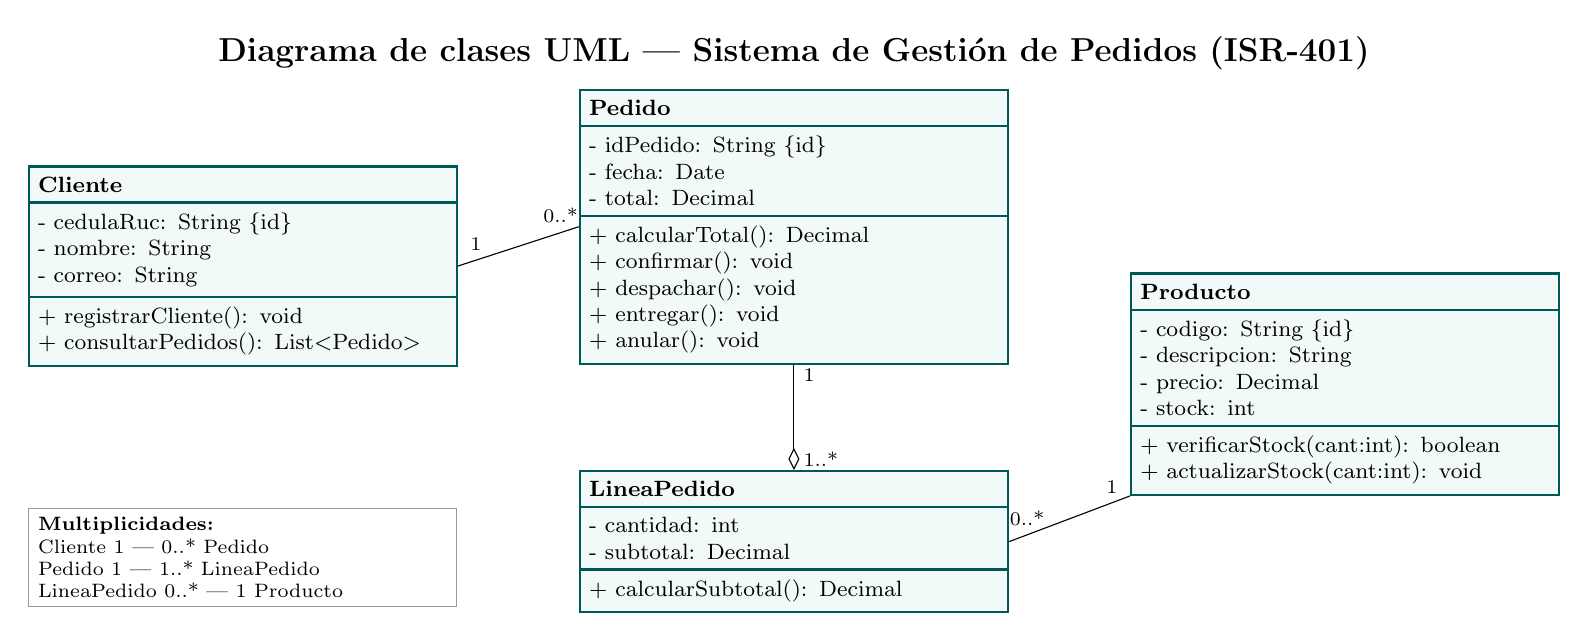
\begin{tikzpicture}[
    class/.style={
        rectangle split, rectangle split parts=3,
        draw=teal!70!black, thick, fill=teal!5,
        rectangle split part align=left,
        text width=5.2cm, font=\footnotesize
    },
    title/.style={font=\bfseries},
    every edge/.style={draw, thick},
    label/.style={font=\scriptsize}
]

% --- Título ---
\node[font=\bfseries\large] at (7,7.7) {Diagrama de clases UML --- Sistema de Gestión de Pedidos (ISR-401)};

% --- Clase Cliente ---
\node[class] (Cliente) at (0,5) {
    \nodepart{one}\textbf{Cliente}
    \nodepart{two}
    - cedulaRuc: String \{id\}\\
    - nombre: String\\
    - correo: String
    \nodepart{three}
    + registrarCliente(): void\\
    + consultarPedidos(): List\textless{}Pedido\textgreater{}
};

% --- Clase Pedido ---
\node[class] (Pedido) at (7,5.5) {
    \nodepart{one}\textbf{Pedido}
    \nodepart{two}
    - idPedido: String \{id\}\\
    - fecha: Date\\
    - total: Decimal
    \nodepart{three}
    + calcularTotal(): Decimal\\
    + confirmar(): void\\
    + despachar(): void\\
    + entregar(): void\\
    + anular(): void
};

% --- Clase LineaPedido ---
\node[class] (LineaPedido) at (7,1.5) {
    \nodepart{one}\textbf{LineaPedido}
    \nodepart{two}
    - cantidad: int\\
    - subtotal: Decimal
    \nodepart{three}
    + calcularSubtotal(): Decimal
};

% --- Clase Producto ---
\node[class] (Producto) at (14,3.5) {
    \nodepart{one}\textbf{Producto}
    \nodepart{two}
    - codigo: String \{id\}\\
    - descripcion: String\\
    - precio: Decimal\\
    - stock: int
    \nodepart{three}
    + verificarStock(cant:int): boolean\\
    + actualizarStock(cant:int): void
};

% --- Asociación Cliente - Pedido ---
\draw[-] (Cliente.east) -- (Pedido.west)
    node[label, pos=0.15, above] {1}
    node[label, pos=0.85, above] {0..*};

% --- Composición Pedido - LineaPedido ---
\draw[-{Diamond[open=false, length=8pt]}] (Pedido.south) -- (LineaPedido.north)
    node[label, pos=0.1, right] {1}
    node[label, pos=0.9, right] {1..*};

% --- Asociación LineaPedido - Producto ---
\draw[-] (LineaPedido.east) -- (Producto.south west)
    node[label, pos=0.15, above] {0..*}
    node[label, pos=0.85, above] {1};

% --- Nota de multiplicidades ---
\node[align=left, font=\scriptsize, draw=black!40, fill=white, text width=5.2cm] at (0,1.3) {
    \textbf{Multiplicidades:}\\
    Cliente 1 --- 0..* Pedido\\
    Pedido 1 --- 1..* LineaPedido\\
    LineaPedido 0..* --- 1 Producto
};

\end{tikzpicture}
\end{document}

% ============================================================

\documentclass[tikz,border=10pt]{standalone}
\usepackage{tikz}
\usetikzlibrary{positioning, shapes.multipart, arrows.meta}

\begin{document}
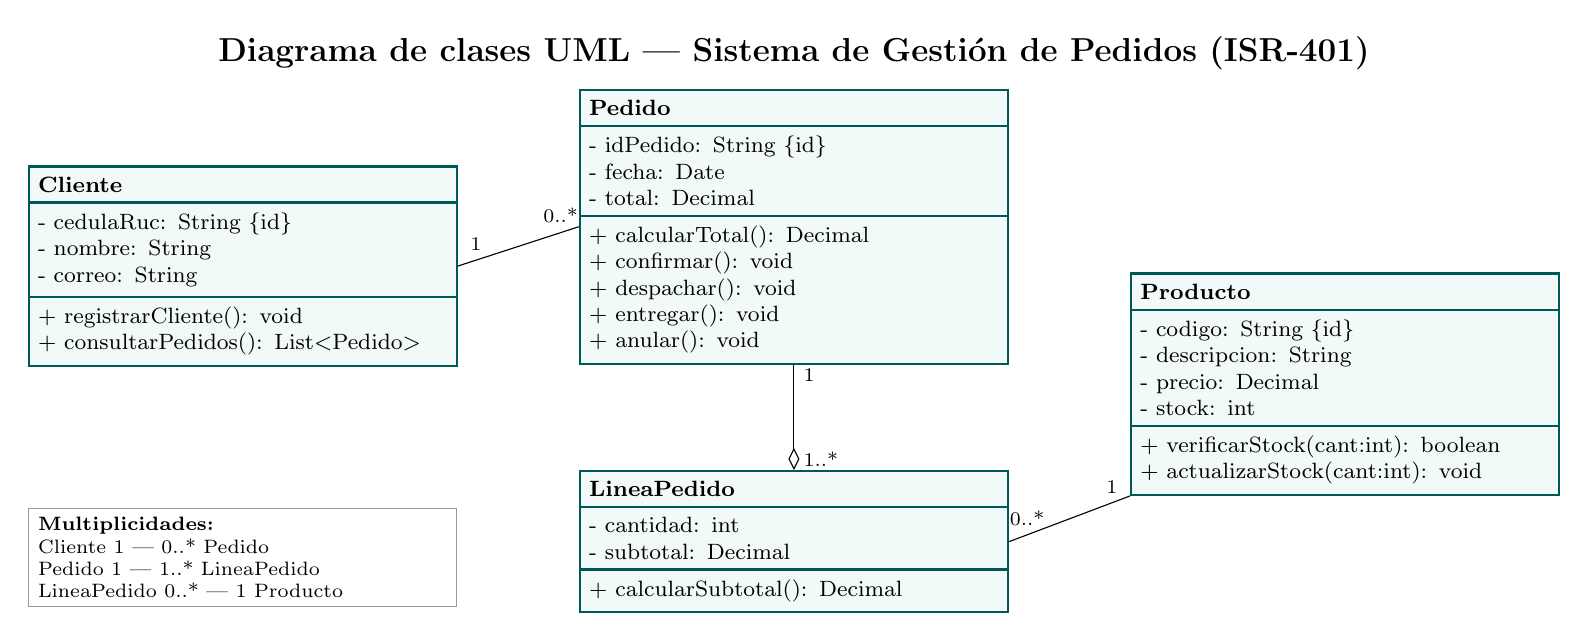
\begin{tikzpicture}[
    class/.style={
        rectangle split, rectangle split parts=3,
        draw=teal!70!black, thick, fill=teal!5,
        rectangle split part align=left,
        text width=5.2cm, font=\footnotesize
    },
    title/.style={font=\bfseries},
    every edge/.style={draw, thick},
    label/.style={font=\scriptsize}
]

% --- Título ---
\node[font=\bfseries\large] at (7,7.7) {Diagrama de clases UML --- Sistema de Gestión de Pedidos (ISR-401)};

% --- Clase Cliente ---
\node[class] (Cliente) at (0,5) {
    \nodepart{one}\textbf{Cliente}
    \nodepart{two}
    - cedulaRuc: String \{id\}\\
    - nombre: String\\
    - correo: String
    \nodepart{three}
    + registrarCliente(): void\\
    + consultarPedidos(): List\textless{}Pedido\textgreater{}
};

% --- Clase Pedido ---
\node[class] (Pedido) at (7,5.5) {
    \nodepart{one}\textbf{Pedido}
    \nodepart{two}
    - idPedido: String \{id\}\\
    - fecha: Date\\
    - total: Decimal
    \nodepart{three}
    + calcularTotal(): Decimal\\
    + confirmar(): void\\
    + despachar(): void\\
    + entregar(): void\\
    + anular(): void
};

% --- Clase LineaPedido ---
\node[class] (LineaPedido) at (7,1.5) {
    \nodepart{one}\textbf{LineaPedido}
    \nodepart{two}
    - cantidad: int\\
    - subtotal: Decimal
    \nodepart{three}
    + calcularSubtotal(): Decimal
};

% --- Clase Producto ---
\node[class] (Producto) at (14,3.5) {
    \nodepart{one}\textbf{Producto}
    \nodepart{two}
    - codigo: String \{id\}\\
    - descripcion: String\\
    - precio: Decimal\\
    - stock: int
    \nodepart{three}
    + verificarStock(cant:int): boolean\\
    + actualizarStock(cant:int): void
};

% --- Asociación Cliente - Pedido ---
\draw[-] (Cliente.east) -- (Pedido.west)
    node[label, pos=0.15, above] {1}
    node[label, pos=0.85, above] {0..*};

% --- Composición Pedido - LineaPedido ---
\draw[-{Diamond[open=false, length=8pt]}] (Pedido.south) -- (LineaPedido.north)
    node[label, pos=0.1, right] {1}
    node[label, pos=0.9, right] {1..*};

% --- Asociación LineaPedido - Producto ---
\draw[-] (LineaPedido.east) -- (Producto.south west)
    node[label, pos=0.15, above] {0..*}
    node[label, pos=0.85, above] {1};

% --- Nota de multiplicidades ---
\node[align=left, font=\scriptsize, draw=black!40, fill=white, text width=5.2cm] at (0,1.3) {
    \textbf{Multiplicidades:}\\
    Cliente 1 --- 0..* Pedido\\
    Pedido 1 --- 1..* LineaPedido\\
    LineaPedido 0..* --- 1 Producto
};

\end{tikzpicture}
\end{document}

% ============================================================

\documentclass[tikz,border=10pt]{standalone}
\usepackage{tikz}
\usetikzlibrary{positioning, shapes.multipart, arrows.meta}

\begin{document}
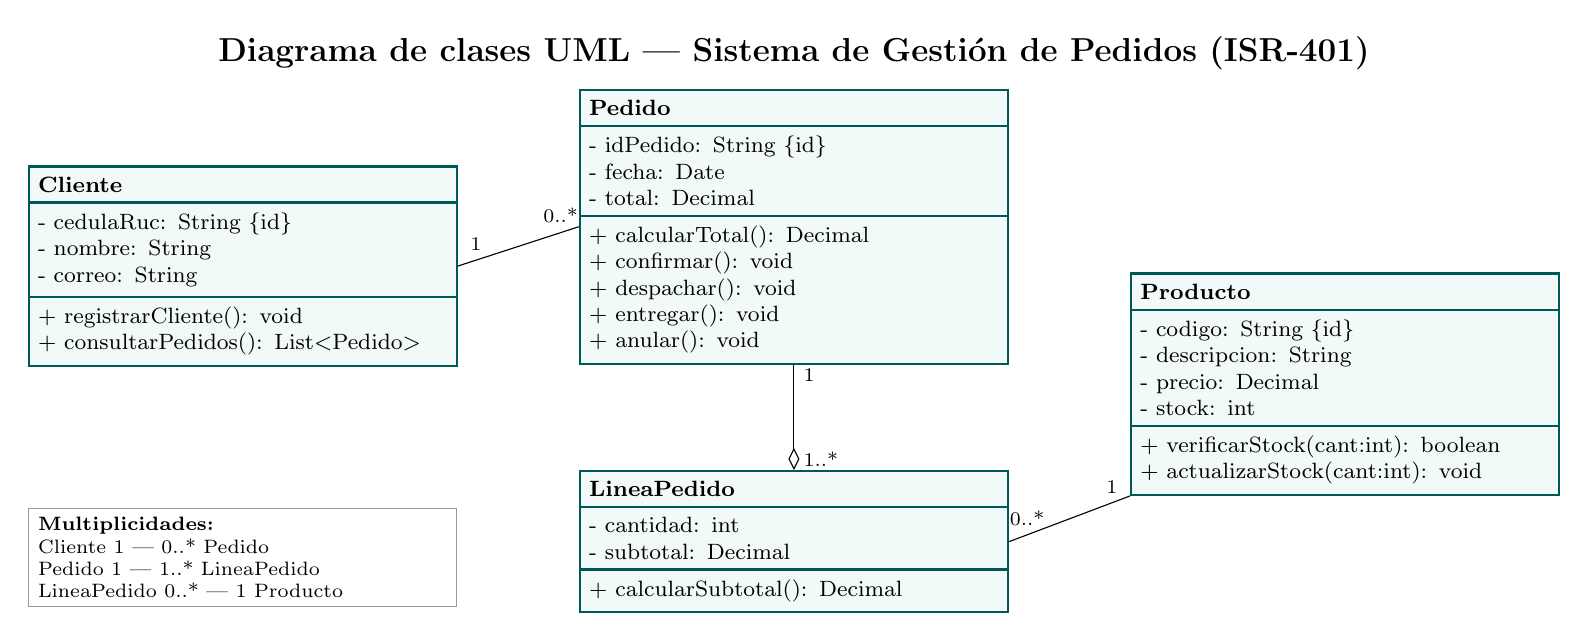
\begin{tikzpicture}[
    class/.style={
        rectangle split, rectangle split parts=3,
        draw=teal!70!black, thick, fill=teal!5,
        rectangle split part align=left,
        text width=5.2cm, font=\footnotesize
    },
    title/.style={font=\bfseries},
    every edge/.style={draw, thick},
    label/.style={font=\scriptsize}
]

% --- Título ---
\node[font=\bfseries\large] at (7,7.7) {Diagrama de clases UML --- Sistema de Gestión de Pedidos (ISR-401)};

% --- Clase Cliente ---
\node[class] (Cliente) at (0,5) {
    \nodepart{one}\textbf{Cliente}
    \nodepart{two}
    - cedulaRuc: String \{id\}\\
    - nombre: String\\
    - correo: String
    \nodepart{three}
    + registrarCliente(): void\\
    + consultarPedidos(): List\textless{}Pedido\textgreater{}
};

% --- Clase Pedido ---
\node[class] (Pedido) at (7,5.5) {
    \nodepart{one}\textbf{Pedido}
    \nodepart{two}
    - idPedido: String \{id\}\\
    - fecha: Date\\
    - total: Decimal
    \nodepart{three}
    + calcularTotal(): Decimal\\
    + confirmar(): void\\
    + despachar(): void\\
    + entregar(): void\\
    + anular(): void
};

% --- Clase LineaPedido ---
\node[class] (LineaPedido) at (7,1.5) {
    \nodepart{one}\textbf{LineaPedido}
    \nodepart{two}
    - cantidad: int\\
    - subtotal: Decimal
    \nodepart{three}
    + calcularSubtotal(): Decimal
};

% --- Clase Producto ---
\node[class] (Producto) at (14,3.5) {
    \nodepart{one}\textbf{Producto}
    \nodepart{two}
    - codigo: String \{id\}\\
    - descripcion: String\\
    - precio: Decimal\\
    - stock: int
    \nodepart{three}
    + verificarStock(cant:int): boolean\\
    + actualizarStock(cant:int): void
};

% --- Asociación Cliente - Pedido ---
\draw[-] (Cliente.east) -- (Pedido.west)
    node[label, pos=0.15, above] {1}
    node[label, pos=0.85, above] {0..*};

% --- Composición Pedido - LineaPedido ---
\draw[-{Diamond[open=false, length=8pt]}] (Pedido.south) -- (LineaPedido.north)
    node[label, pos=0.1, right] {1}
    node[label, pos=0.9, right] {1..*};

% --- Asociación LineaPedido - Producto ---
\draw[-] (LineaPedido.east) -- (Producto.south west)
    node[label, pos=0.15, above] {0..*}
    node[label, pos=0.85, above] {1};

% --- Nota de multiplicidades ---
\node[align=left, font=\scriptsize, draw=black!40, fill=white, text width=5.2cm] at (0,1.3) {
    \textbf{Multiplicidades:}\\
    Cliente 1 --- 0..* Pedido\\
    Pedido 1 --- 1..* LineaPedido\\
    LineaPedido 0..* --- 1 Producto
};

\end{tikzpicture}
\end{document}

% ============================================================

\documentclass[tikz,border=10pt]{standalone}
\usepackage{tikz}
\usetikzlibrary{positioning, shapes.multipart, arrows.meta}

\begin{document}
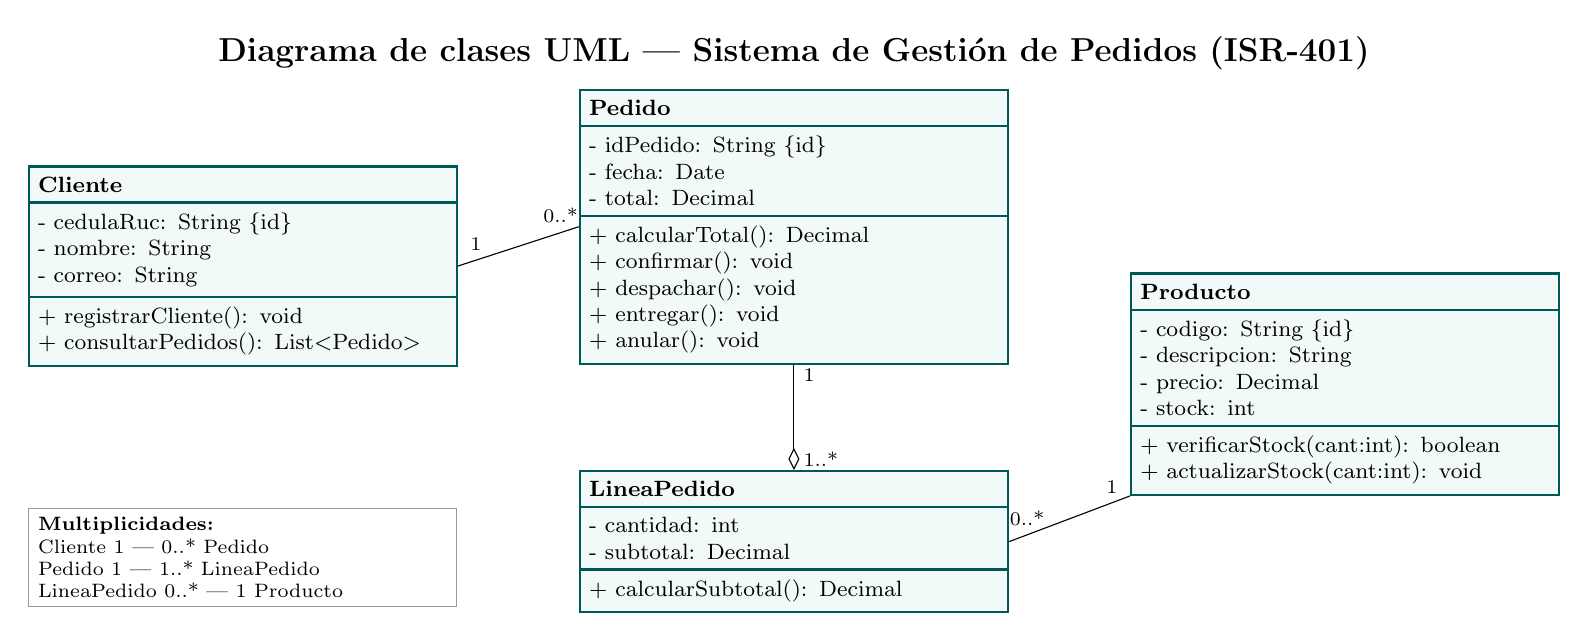
\begin{tikzpicture}[
    class/.style={
        rectangle split, rectangle split parts=3,
        draw=teal!70!black, thick, fill=teal!5,
        rectangle split part align=left,
        text width=5.2cm, font=\footnotesize
    },
    title/.style={font=\bfseries},
    every edge/.style={draw, thick},
    label/.style={font=\scriptsize}
]

% --- Título ---
\node[font=\bfseries\large] at (7,7.7) {Diagrama de clases UML --- Sistema de Gestión de Pedidos (ISR-401)};

% --- Clase Cliente ---
\node[class] (Cliente) at (0,5) {
    \nodepart{one}\textbf{Cliente}
    \nodepart{two}
    - cedulaRuc: String \{id\}\\
    - nombre: String\\
    - correo: String
    \nodepart{three}
    + registrarCliente(): void\\
    + consultarPedidos(): List\textless{}Pedido\textgreater{}
};

% --- Clase Pedido ---
\node[class] (Pedido) at (7,5.5) {
    \nodepart{one}\textbf{Pedido}
    \nodepart{two}
    - idPedido: String \{id\}\\
    - fecha: Date\\
    - total: Decimal
    \nodepart{three}
    + calcularTotal(): Decimal\\
    + confirmar(): void\\
    + despachar(): void\\
    + entregar(): void\\
    + anular(): void
};

% --- Clase LineaPedido ---
\node[class] (LineaPedido) at (7,1.5) {
    \nodepart{one}\textbf{LineaPedido}
    \nodepart{two}
    - cantidad: int\\
    - subtotal: Decimal
    \nodepart{three}
    + calcularSubtotal(): Decimal
};

% --- Clase Producto ---
\node[class] (Producto) at (14,3.5) {
    \nodepart{one}\textbf{Producto}
    \nodepart{two}
    - codigo: String \{id\}\\
    - descripcion: String\\
    - precio: Decimal\\
    - stock: int
    \nodepart{three}
    + verificarStock(cant:int): boolean\\
    + actualizarStock(cant:int): void
};

% --- Asociación Cliente - Pedido ---
\draw[-] (Cliente.east) -- (Pedido.west)
    node[label, pos=0.15, above] {1}
    node[label, pos=0.85, above] {0..*};

% --- Composición Pedido - LineaPedido ---
\draw[-{Diamond[open=false, length=8pt]}] (Pedido.south) -- (LineaPedido.north)
    node[label, pos=0.1, right] {1}
    node[label, pos=0.9, right] {1..*};

% --- Asociación LineaPedido - Producto ---
\draw[-] (LineaPedido.east) -- (Producto.south west)
    node[label, pos=0.15, above] {0..*}
    node[label, pos=0.85, above] {1};

% --- Nota de multiplicidades ---
\node[align=left, font=\scriptsize, draw=black!40, fill=white, text width=5.2cm] at (0,1.3) {
    \textbf{Multiplicidades:}\\
    Cliente 1 --- 0..* Pedido\\
    Pedido 1 --- 1..* LineaPedido\\
    LineaPedido 0..* --- 1 Producto
};

\end{tikzpicture}
\end{document}
